\documentclass{article}
\usepackage[utf8]{inputenc}
\usepackage[options ]{algorithm2e}
\usepackage{algorithmic}
\usepackage{algorithm}

\usepackage[english]{babel}
\usepackage[utf8]{inputenc}
\usepackage{amsmath}
\usepackage{amsfonts}
\usepackage{graphicx}
\usepackage[colorinlistoftodos]{todonotes}
\usepackage{algorithm}
\usepackage{algpseudocode}

\title{The Dining Philosophers problem}
\author{Diaconescu Bogdan-Florin\\ CR 3.2 A, Anul 3}

\usepackage{natbib}
\usepackage{graphicx}

\begin{document}
\maketitle
\newpage
\section{Problem statement}
\hspace{0.5 cm}
There is a group of philosophers (usually 5) who eat together at a round table. There are forks placed between the philosophers. Philosophers spend their time either thinking or eating. In order to eat, a philosopher must pick up exactly two forks, one on his immediate left, and the other on his immediate right. When he is done eating, he will put his forks down so that his neighbors may use them, and he thinks again.

\section{Implementation/Solution}
\hspace{0.5 cm}
The programming problem is to construct a simulation that will allow philosophers to move between their eating and thinking states while properly controlling the forks. 

 \hspace{0.5 cm}
 A typical solution has each philosopher doing something like this:
 
\begin{algorithm} 
\caption{}
\begin{algorithmic}[1]

\WHILE{true}
\STATE busy thinking
\STATE wait for left fork
\STATE wait for right fork
\STATE busy eating
\STATE drop left fork
\STATE drop right fork
\ENDWHILE

\end{algorithmic}
\end{algorithm}
 
\hspace{0.5 cm}
To solve this problem, I created a generic class "Channel <T>" that has 2 functions: "synchronized void send(T mes)" and "synchronized T receive()". I defined a int variable ready that it's used to indicated the message's status. When ready = 0, the message can be sent, then the ready variable is incremented. When ready = 1, the message can be receive, then the ready variable is decremented. Each processes announces the other processes when the message has been sent or received using the function notifyAll(). 

\hspace{0.5 cm}
Fork class extends Thread and has a function "void run()". In this function, for each element of forks array, call send(true) and receive() in an infinite while loop. -	Forks are implemented trough independent processes which communicate with the philosophers using channels. A philosopher communicates with a fork i using the channel Forks i (that represents the left fork) and with a fork i+1 (right fork) using the channel Forks i+1.

\hspace{0.5 cm}
 In Philosopher class we create the Philosopher. When both forks are 	available, message transmitted through the channel using the method get, 	the philosopher eats.
 
 \hspace{0.5 cm}
 Dining class corresponds to the Main class, where the philosopher are instantiated. Each philosopher gets a name, the index of the right and left forks and a forks instance which represents the channel. The threads are 	launched in execution.
 
\section{Experimental data and outputs}
\hspace{0.5 cm}

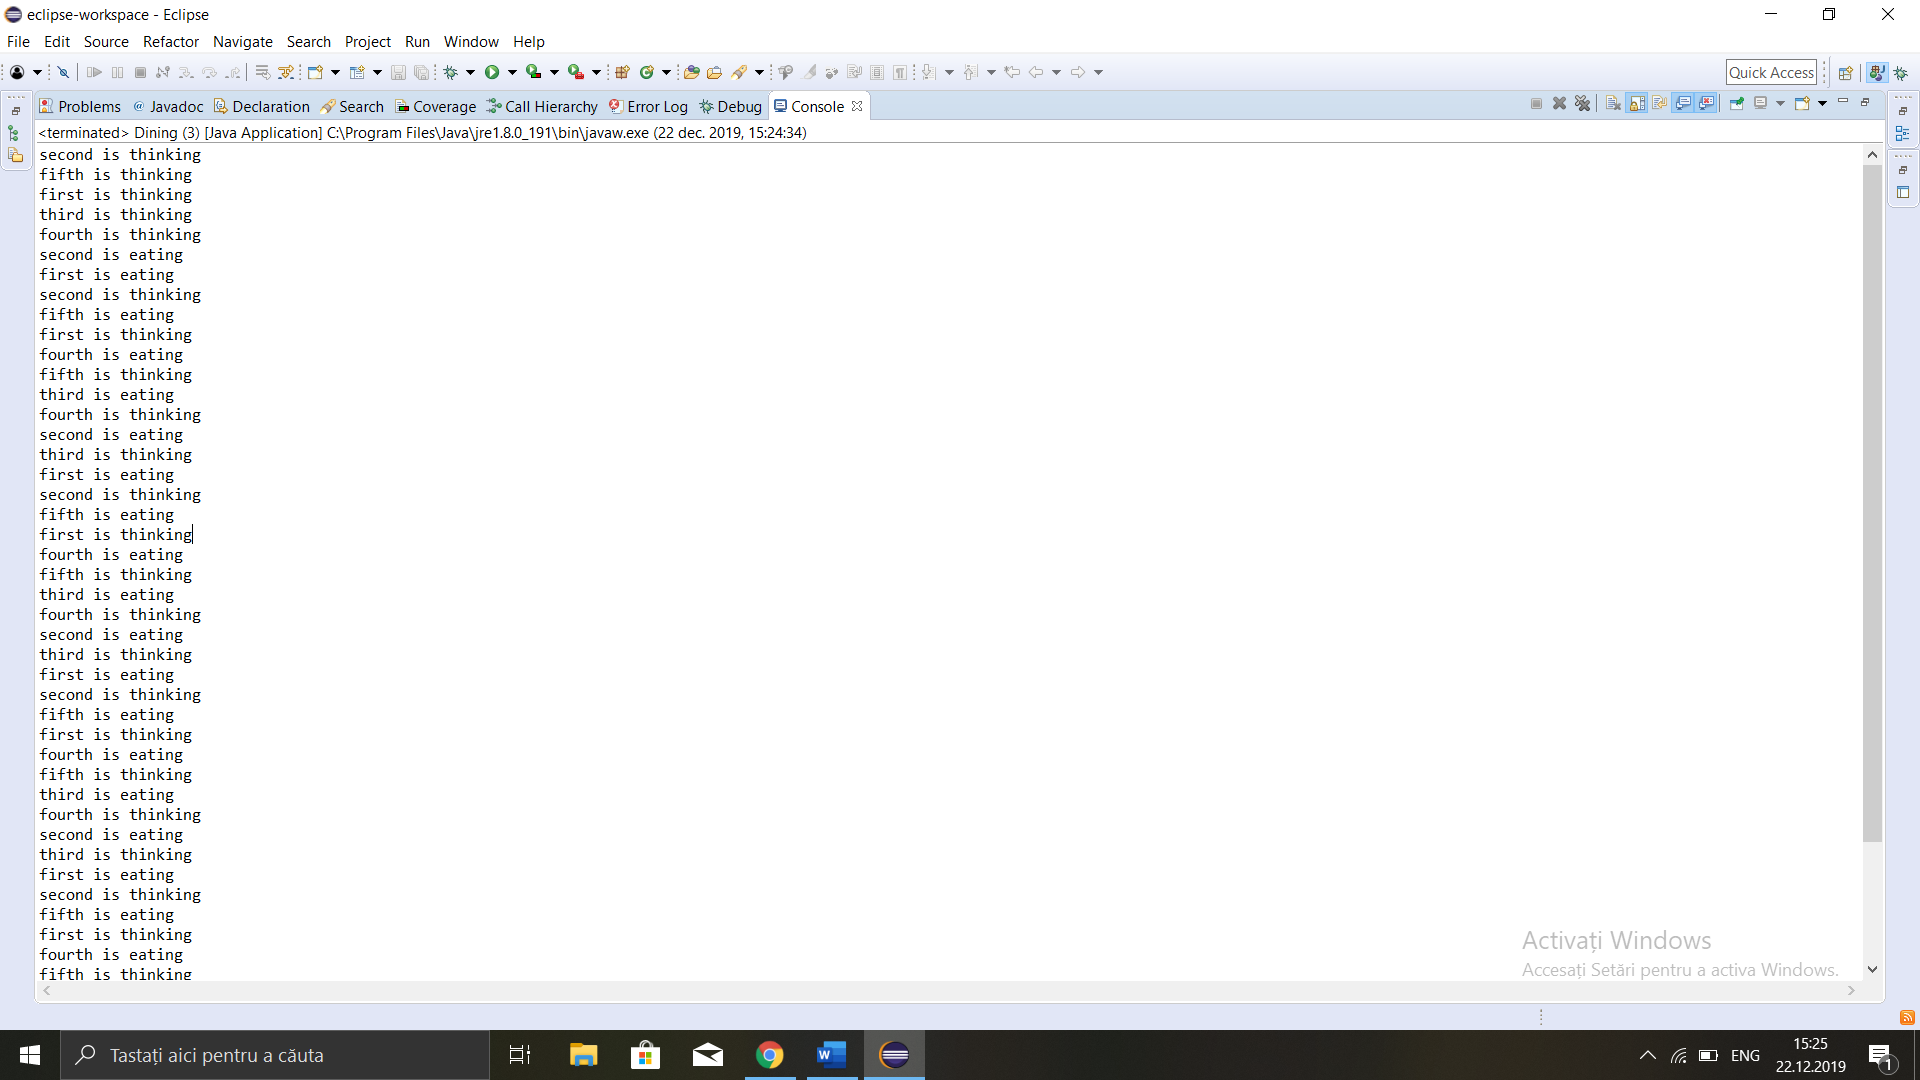
\includegraphics{Channels.png}

 
\section{Conclusion}
\hspace{0.5 cm} 
I solve this problem using channels. In other words, the forks communicate with the philosophers trough the channels. When a fork sends a message it means that it is available. When the philosopher sends a message it means that the fork was released. 
\end{document}
